\subsubsection{Endelige eksperiment for PINN\_z}
Den endelige trænede model for PINN\_z er bestemt ud fra resultaterne af udforskningen af modelarkitektur og hyperparametre i kapitel \ref{ch5_1_design_af_eksperiment}.
Her er hyperparametrene sat til at være: learning rate $10^{-4}$, hidden dimension (8, 8), aktiveringsfunktion er SiLU, 
antal lag 2, data loss vægtes med 0.25, PDE loss vægtes med $10^{4}$, input er hele x rækken, med en z bredde på 1 nabe celle i begge rætninger,
batch størrelse på 1024, træning, validering og test split på $[0, 80\%]$, $(80\%, 90\%]$ og $(90\%, 100\%]$,
hvor \texttt{Alexander\_e} splittes med tidsrække og \texttt{Alexander\_phi\_0} splittes med random sample, 200 epochs,
og early stopping patience på 30 og min\_delta på 0.0.
Denne opsætning er valgt, fordi den i den forrige udforskning gav den bedste kombination af lav test loss og stabil træning.

Der blev kørt 3 eksperimenter med denne arkitektur hvilket gav følgende træning, validering og test kurver:


\begin{figure}[H]
    \centering
    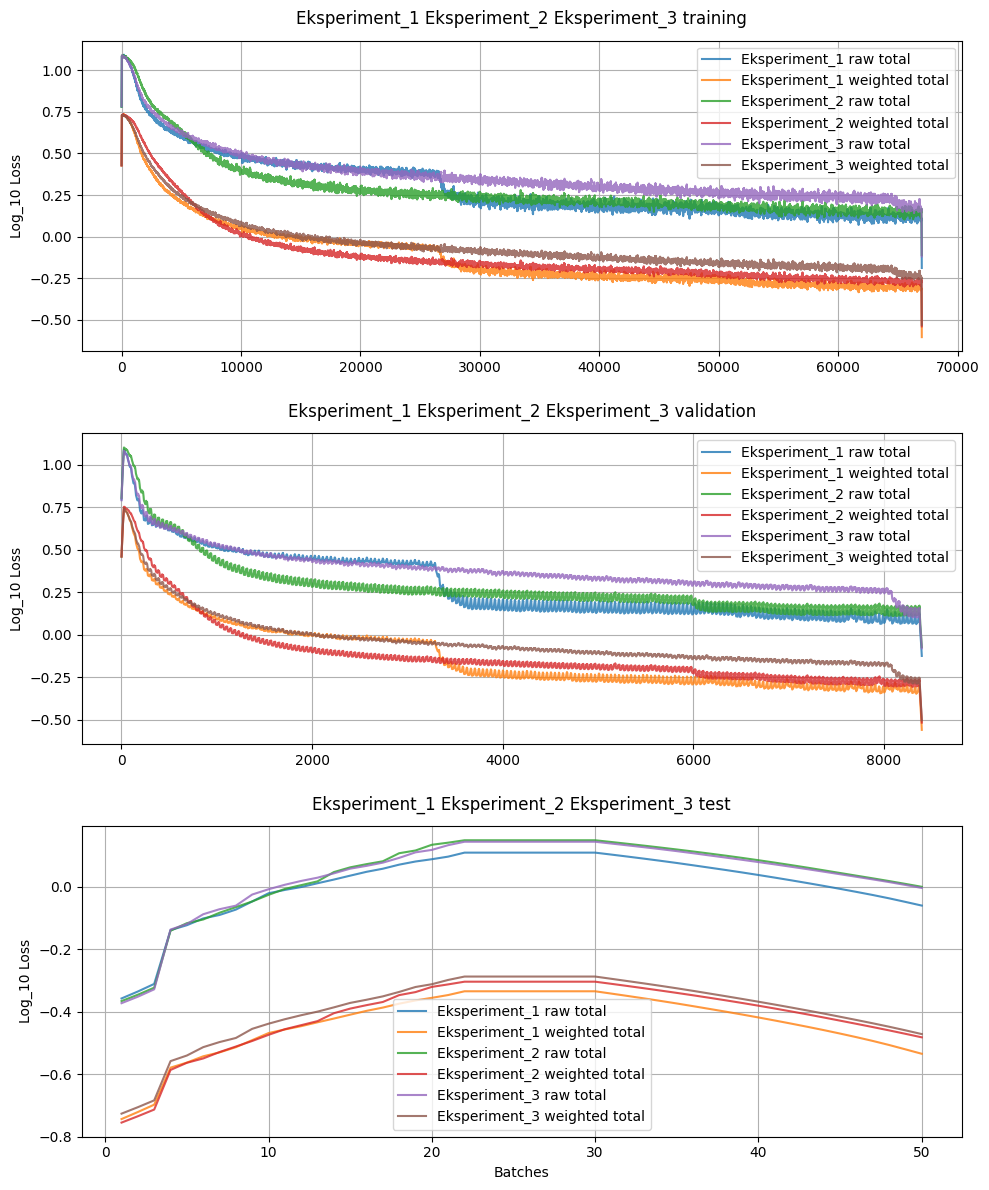
\includegraphics[width=0.8\textwidth]{figures/Final_pinn_z.png}
    \caption{Endelige eksperimenter for PINN\_z med 3 forskellige random seeds, vægtet og uvægtet loss, og moving average med vindue størrelse 50.}
    \label{fig:endelige-eksperimenter-pinn-z}
\end{figure}

\begin{figure}[H]
    \centering
    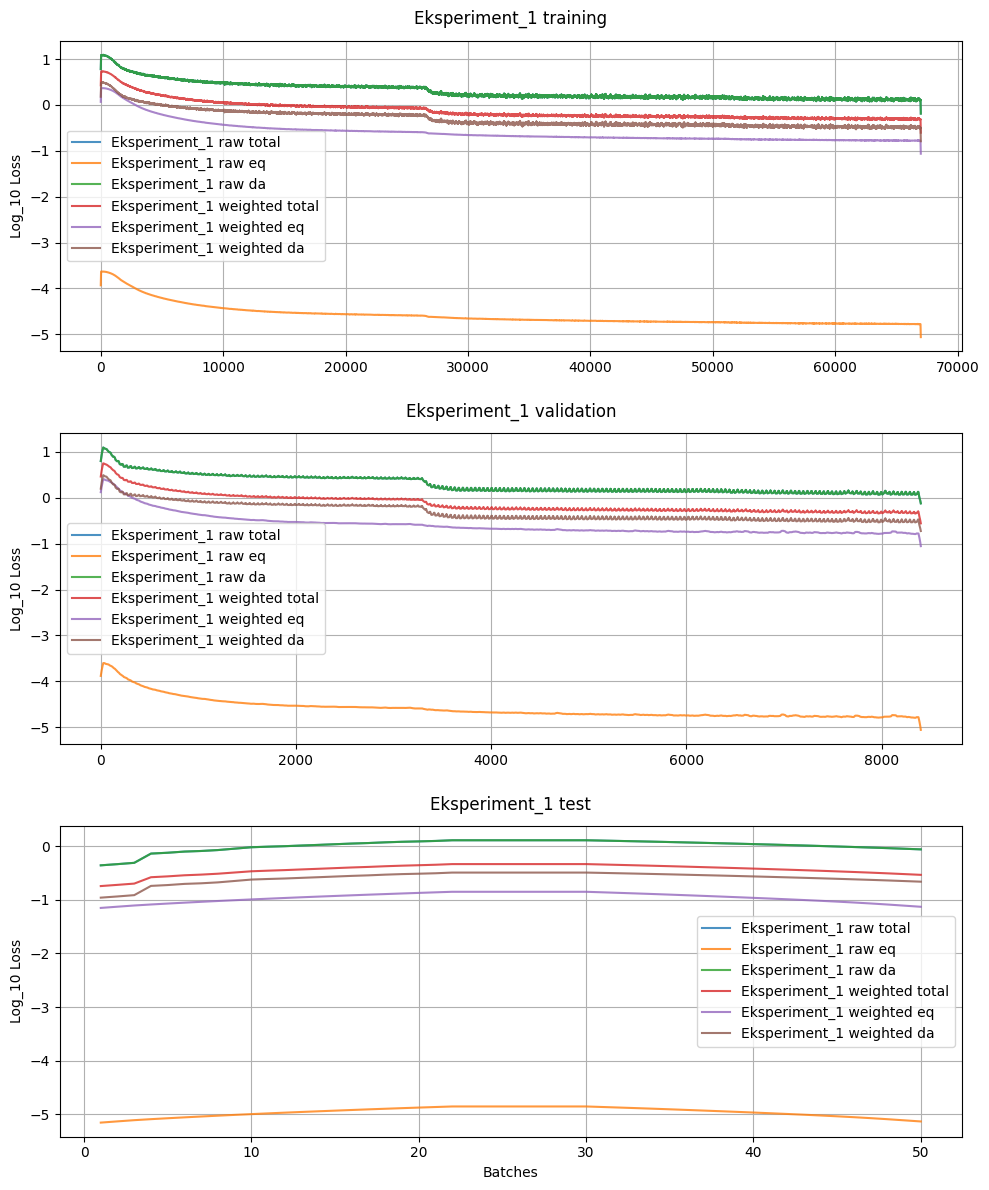
\includegraphics[width=0.8\textwidth]{figures/Final_pinn_z_composite.png}
    \caption{Endelige eksperiment for PINN\_z, Eksperiment 1, med vægtede og uvægtede losses for total, data og PDE (eq), samt moving average med vindue størrelse 50.}
    \label{fig:endelige-eksperiment-pinn-z-composite}
\end{figure}


På figur \ref{fig:endelige-eksperimenter-pinn-z} ses at alle 3 eksperimenter har en meget lignende udvikling og konvergere mod samme
resultat. 
På figur \ref{fig:endelige-eksperiment-pinn-z-composite} ses det ikke tydeligt men for uvægtede loss, ligger data og total loss næsten oven i hinanden, 
imens PDE (eq) ligger helt i bunden. For de vægtede loss, ligger data og PDE (eq) loss næsten oven i hinanden, hvilket betyder de vægtes næsten lige meget og giver 
meget stabil træning. Her til skal det siges at ingen af modellerne konvergerede helt inden for de 200 epochs.
Det tyder på, at den valgte vægtning gjorde optimeringen mere robust uden helt at fjerne behovet for længere træning.

\begin{figure}[H]
    \centering
    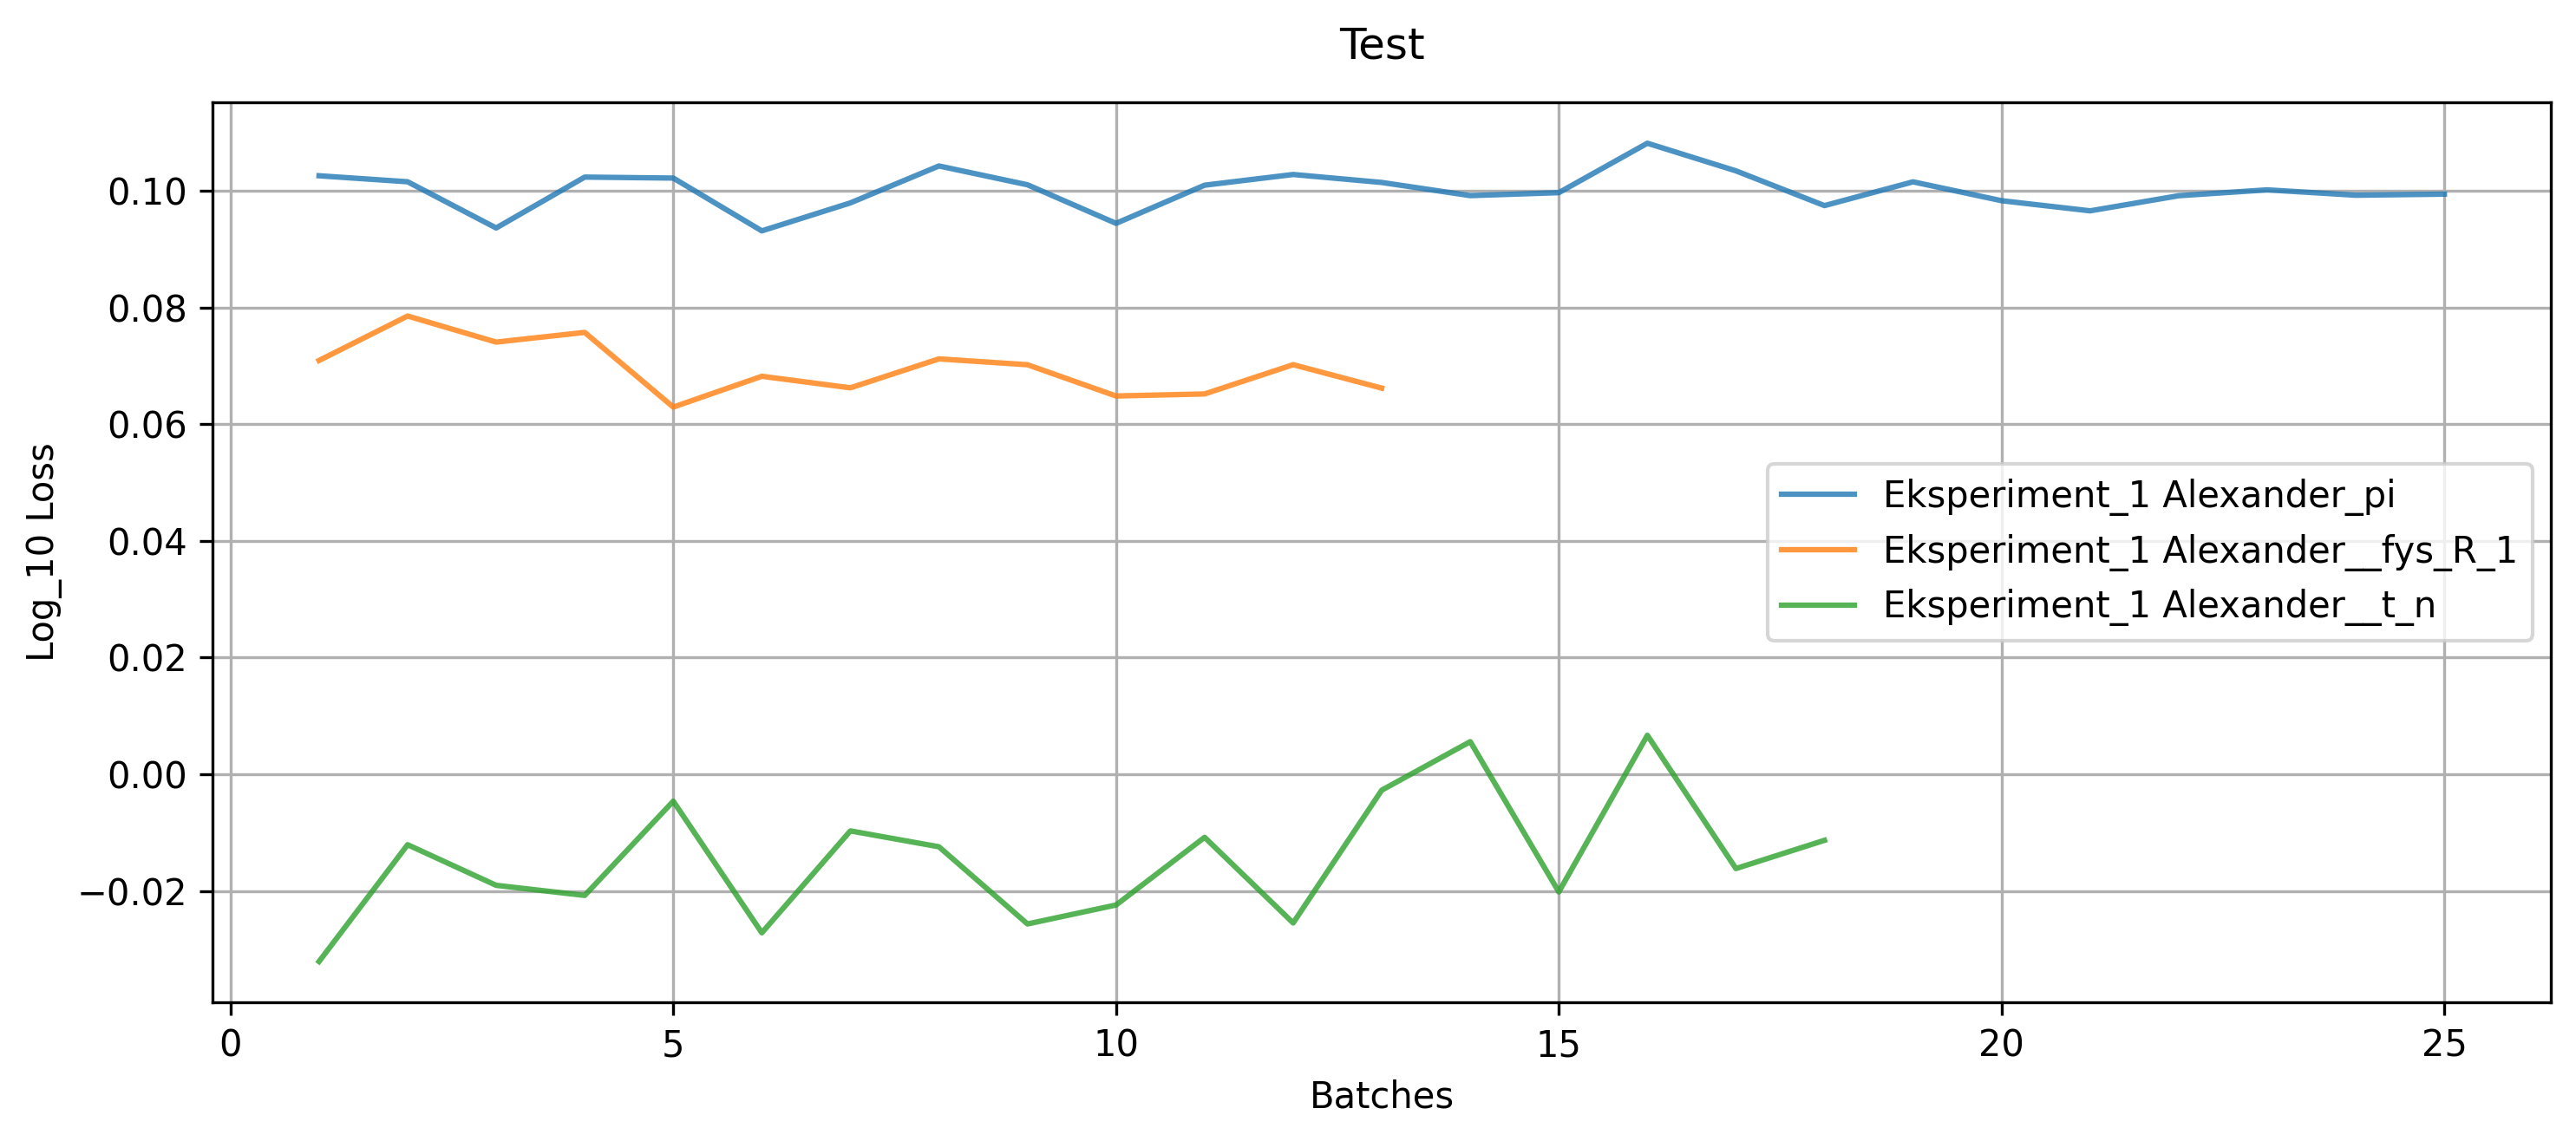
\includegraphics[width=0.8\textwidth]{figures/total_raw_ex1.png}\par\medskip
    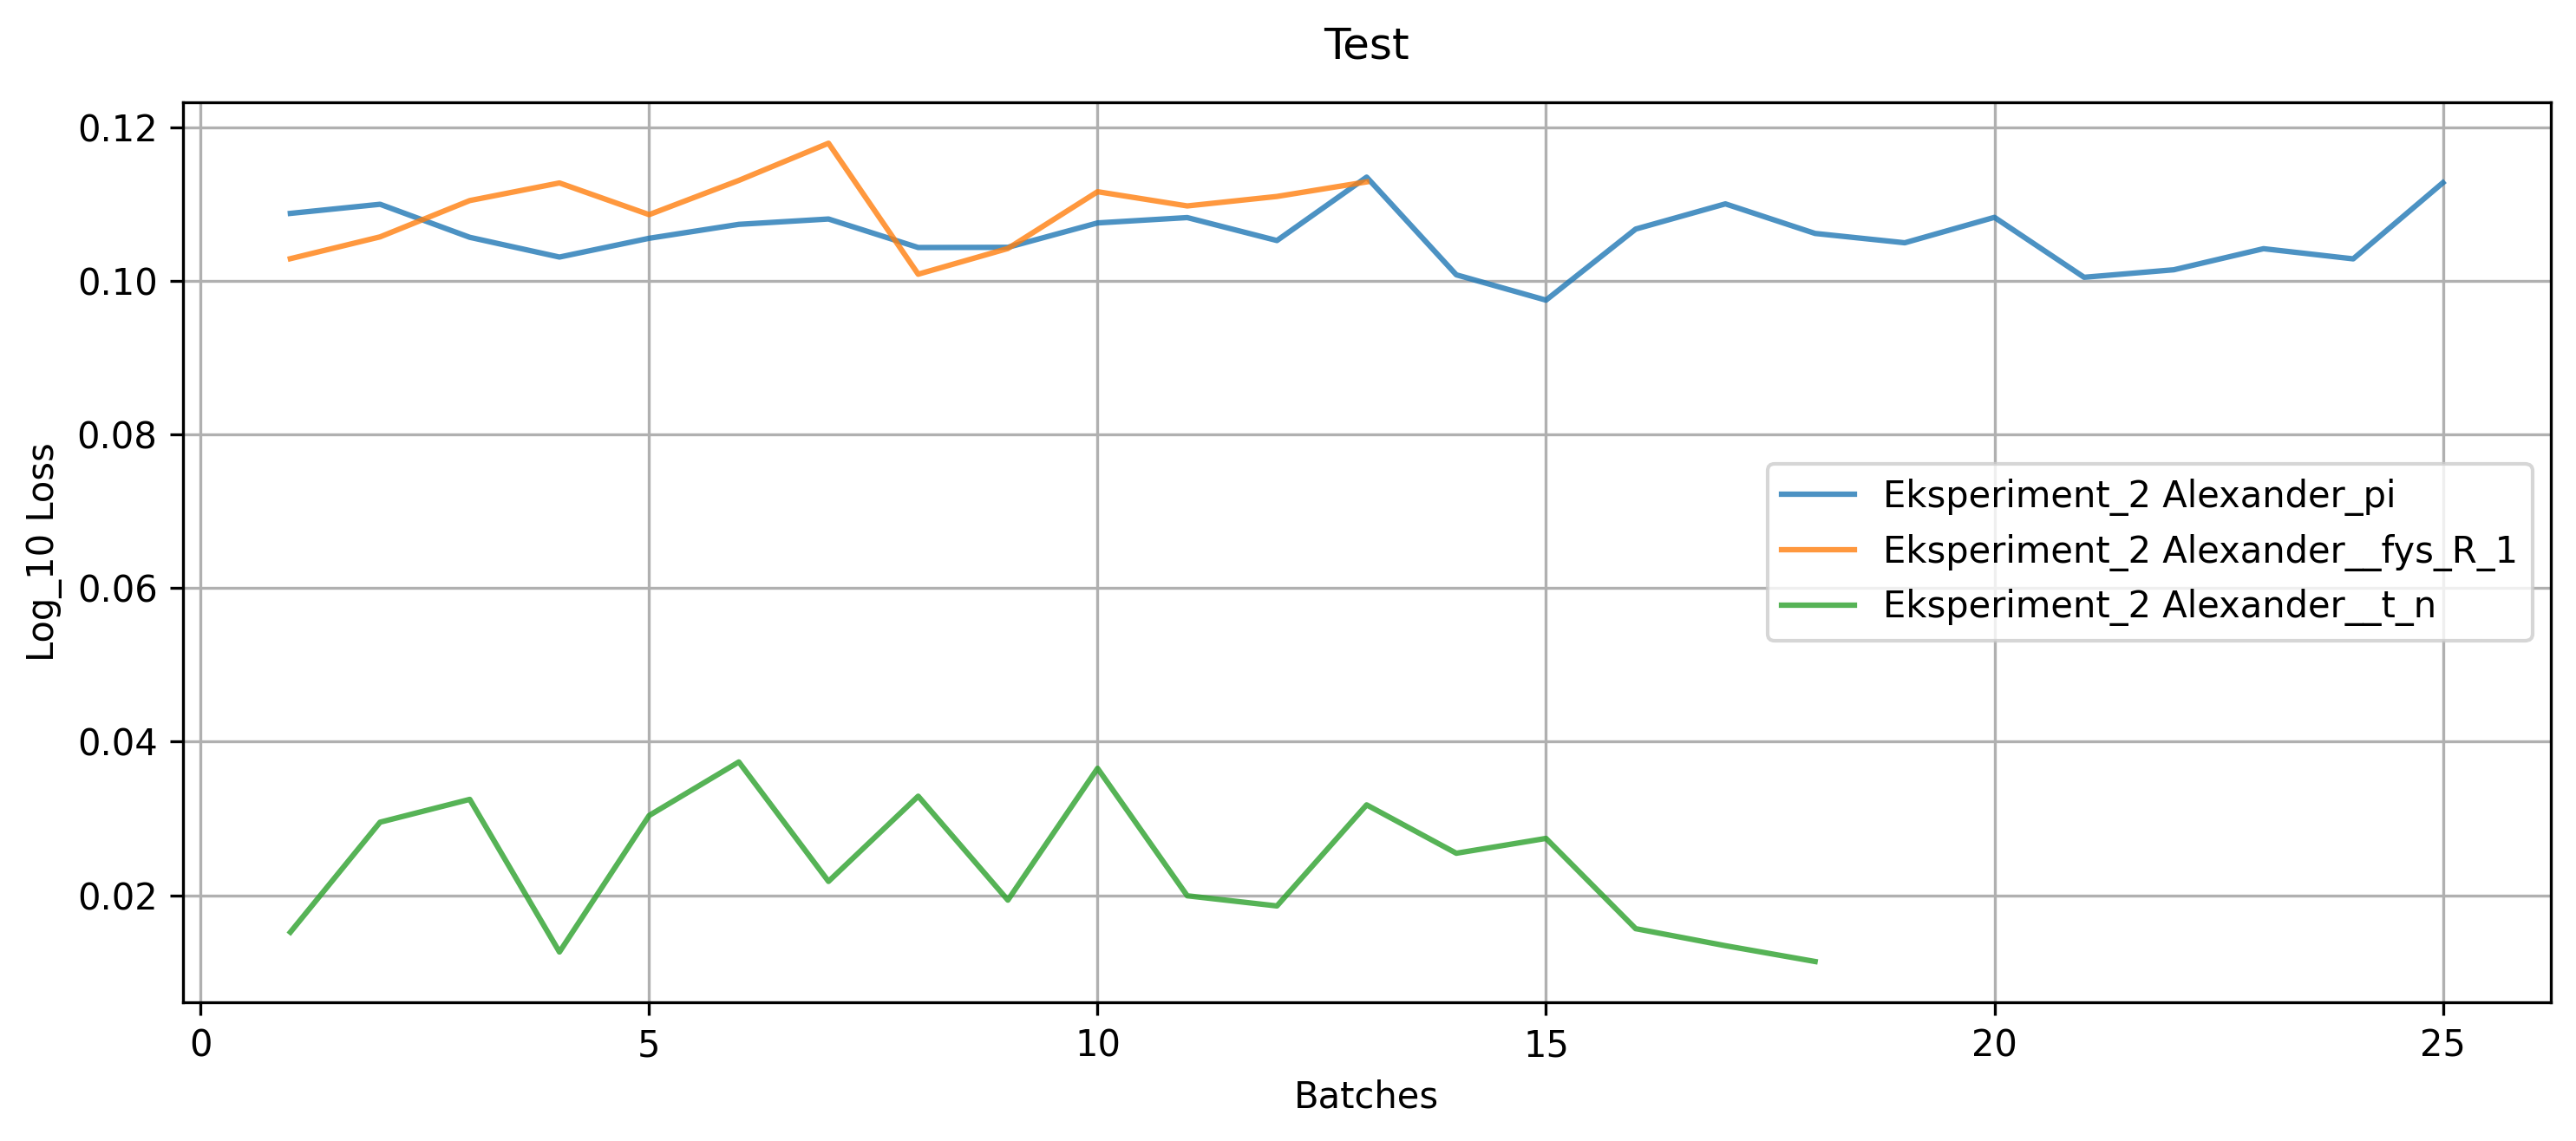
\includegraphics[width=0.8\textwidth]{figures/total_raw_ex2.png}\par\medskip
    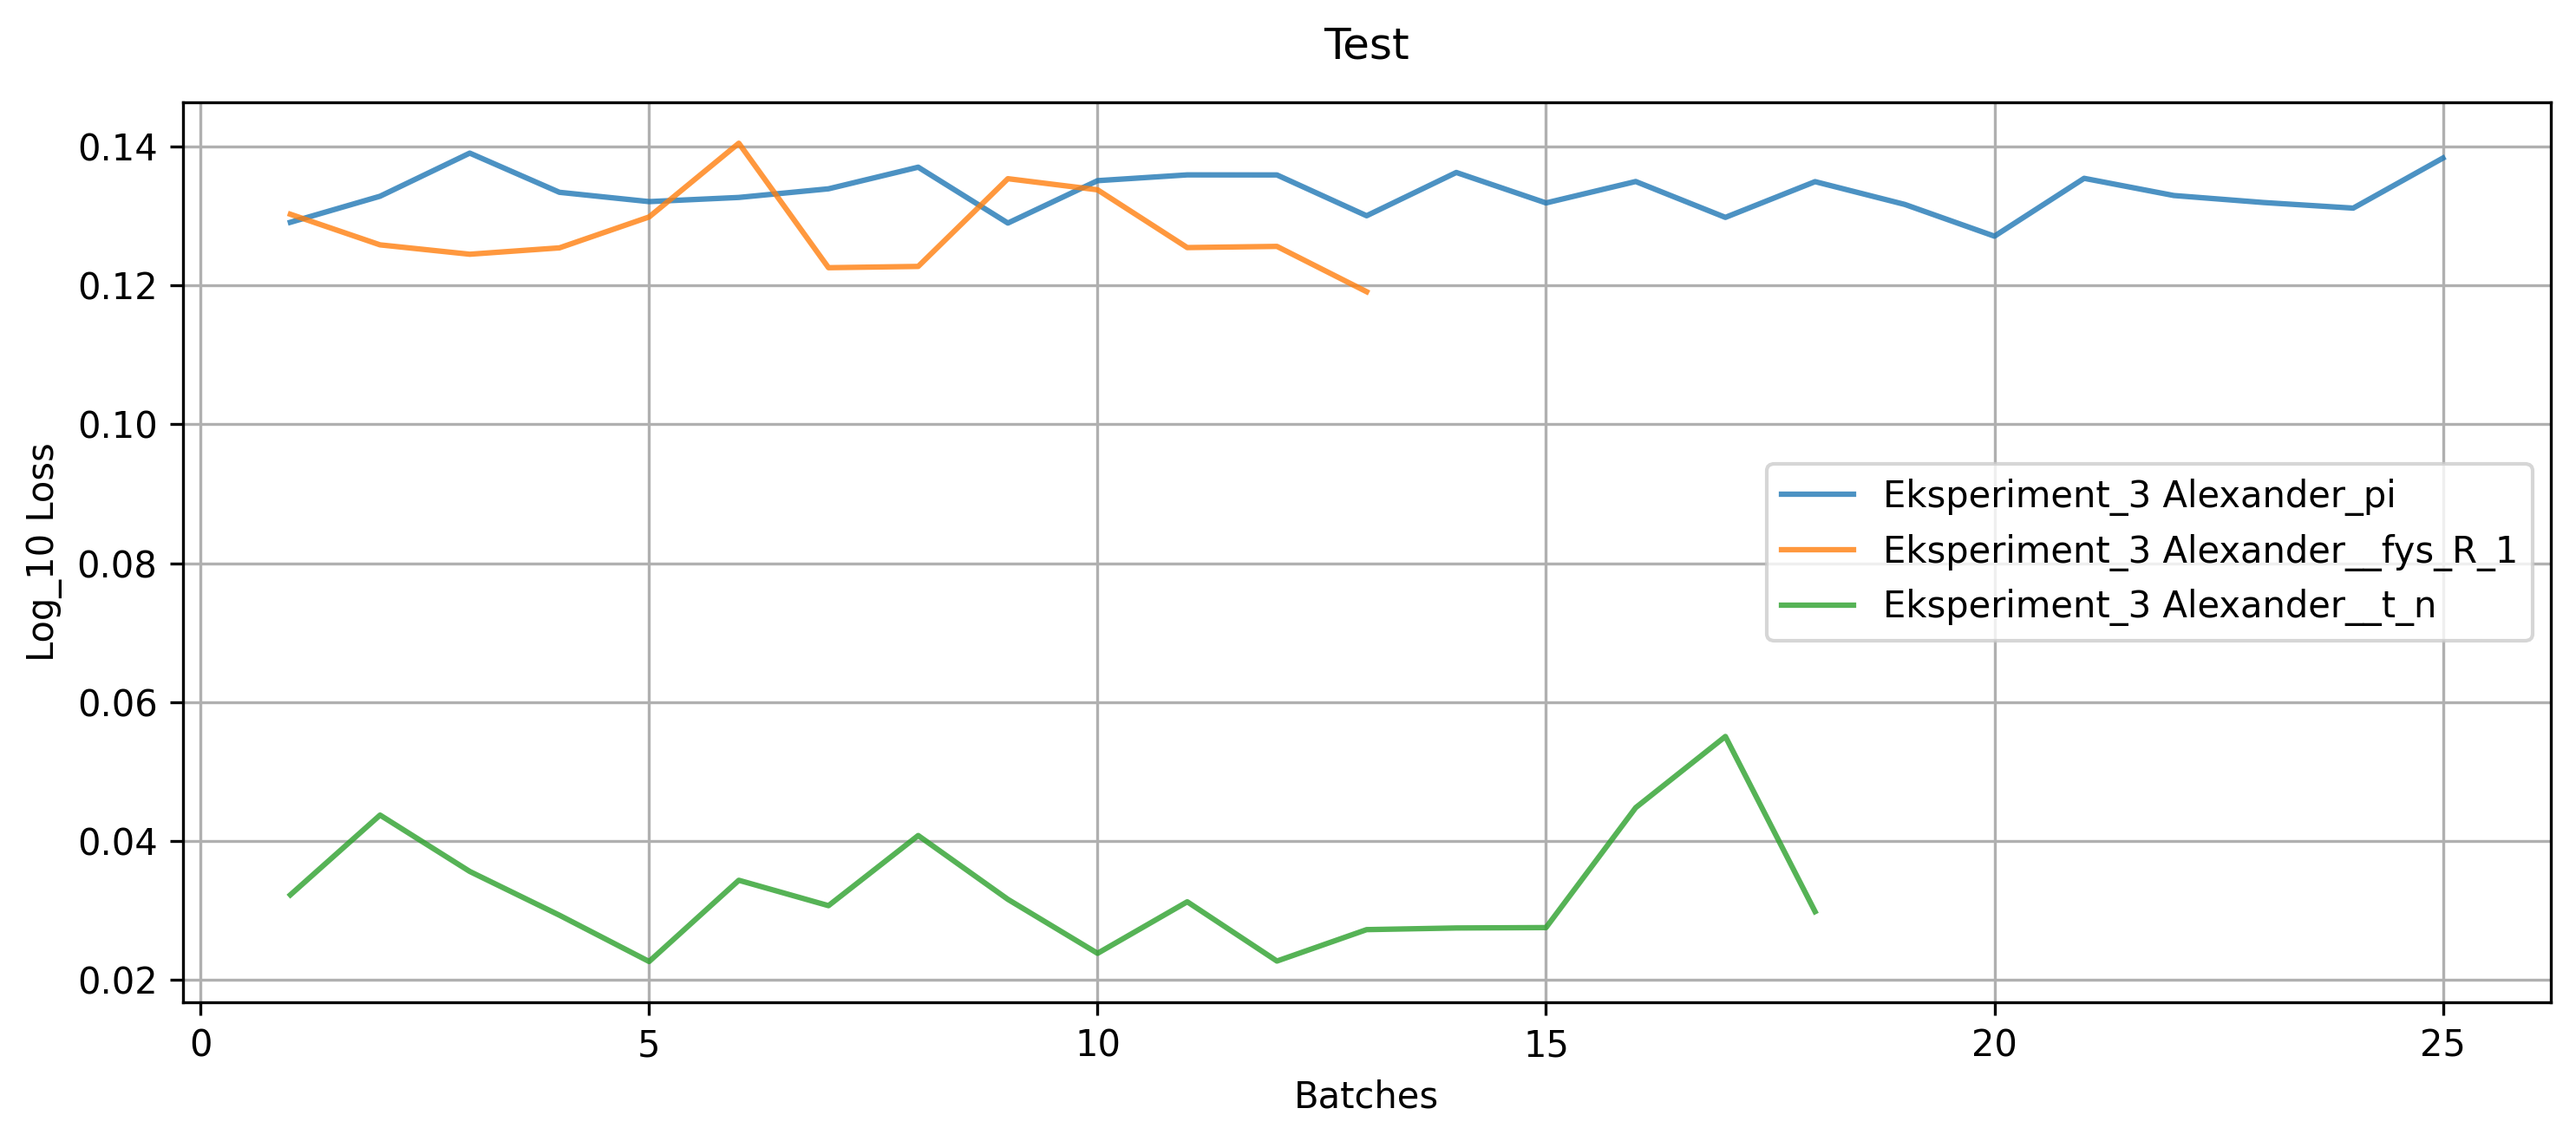
\includegraphics[width=0.8\textwidth]{figures/total_raw_ex3.png}
    \caption{Total uvægtet loss på testdatasættene for Eksperiment 1, 2 og 3, alle med batchstørrelse 1024.}
    \label{fig:endelige-test-paa-testdatasaettet-for-eksperiment-1-2-3}
\end{figure}


På figur \ref{fig:endelige-test-paa-testdatasaettet-for-eksperiment-1-2-3}, ses det at alle 3 eksperimenter har ens test kurver for alle ukendte datasæt.
Alle modeller sig bedst på datasættet med længere tidsstep, frem for kendt og ukend fysik. Dette kan være tegn på overfitting af data.
Da dette er uvægtet loss, har PDE loss også en meget lav loss.
Det samlede billede er derfor, at modellen generaliserer ens på tværs af seeds, men stadig har sværere ved ændret fysik end ved ændret tidsdiskretisering.



Det endelige billede ser nogenlunde således ud:
\begin{figure}[H]
    \centering
    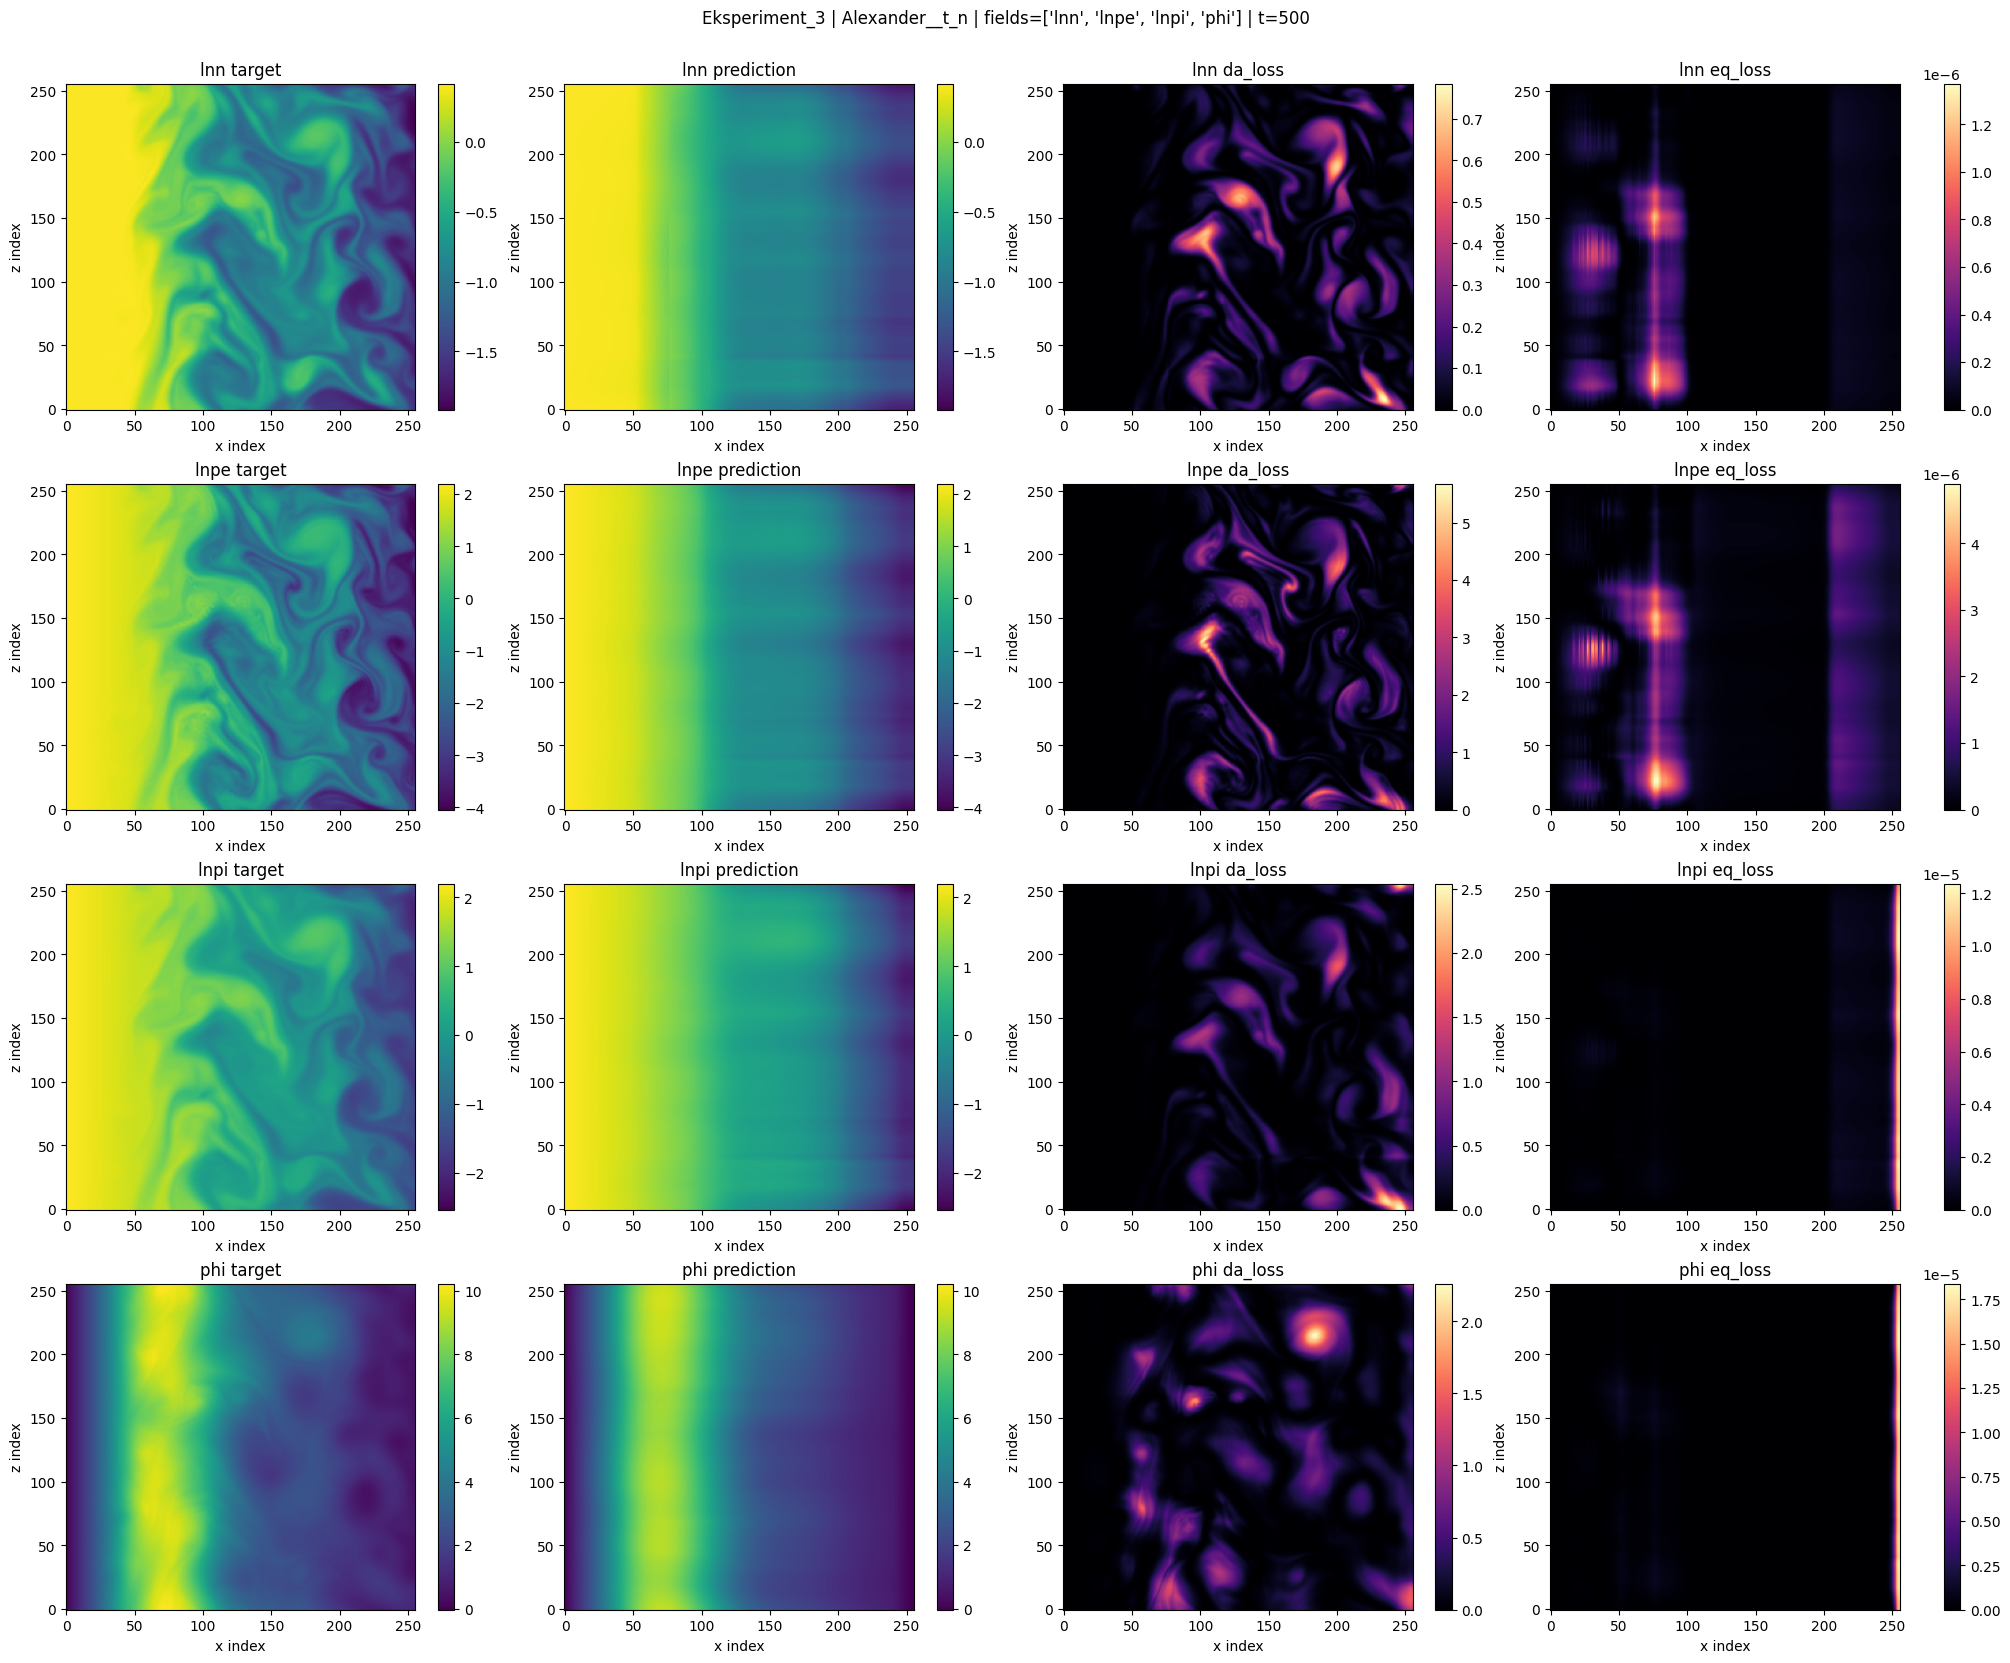
\includegraphics[width=1\textwidth]{figures/endelige_resultatet.png}
    \caption{Modellens mål at forudsige \texttt{Alexander\_\_t\_n} ved \texttt{t\_idx = 500} og \texttt{t\_fys = 12500}, sammenlignet med det faktiske resultat, data loss og PDE (eq) loss.}
    \label{fig:endelige-test-paa-testdatasaettet-for-eksperiment-1}
\end{figure}


Selvom modellen ikke rammer dynamikkerne i data'en serlig godt, rammer den fysikken til yderst højt nøjagtighed da modellen vægter PDE (eq)
loss ekstremt højt. Derofor burde det være muligt at ofre PDE (eq) loss  og træningsstabilitet for data nøjagtighed.


\subsubsection{Endelige eksperiment for PINN}
Da PINN havde problemer med træning sættes model arkitekturen tils at være:
For lag 1 var hidden dimension 256 og aktiveringsfunktion SiLU,
for lag 2 var hidden dimension 128 og aktiveringsfunktion SiLU,
for lag 3 var hidden dimension 128 og aktiveringsfunktion SiLU,
for lag 4 var hidden dimension 128 og aktiveringsfunktion Tanh,
for lag 5 var hidden dimension 64 og aktiveringsfunktion SiLU. Hyper parametrene var for denne model:
Træningsdatasæt var \texttt{Alexander\_e}, med tidsække split med 80\% træning 10\%validering og 10\%test, 1 epoch, learning rate på $10^{-4}$, 
batch størrelse på 4000, data loss vægtet med 500 og PDE (eq) loss vægtet med $10^{3}$, og initial og rand betingelser vægtet 1.
Dette gav trænings, validerings og test kurver som ses på figur \ref{fig:endelige-traening-composite-loss-for-pinn}. 
\begin{figure}[H]
    \centering
    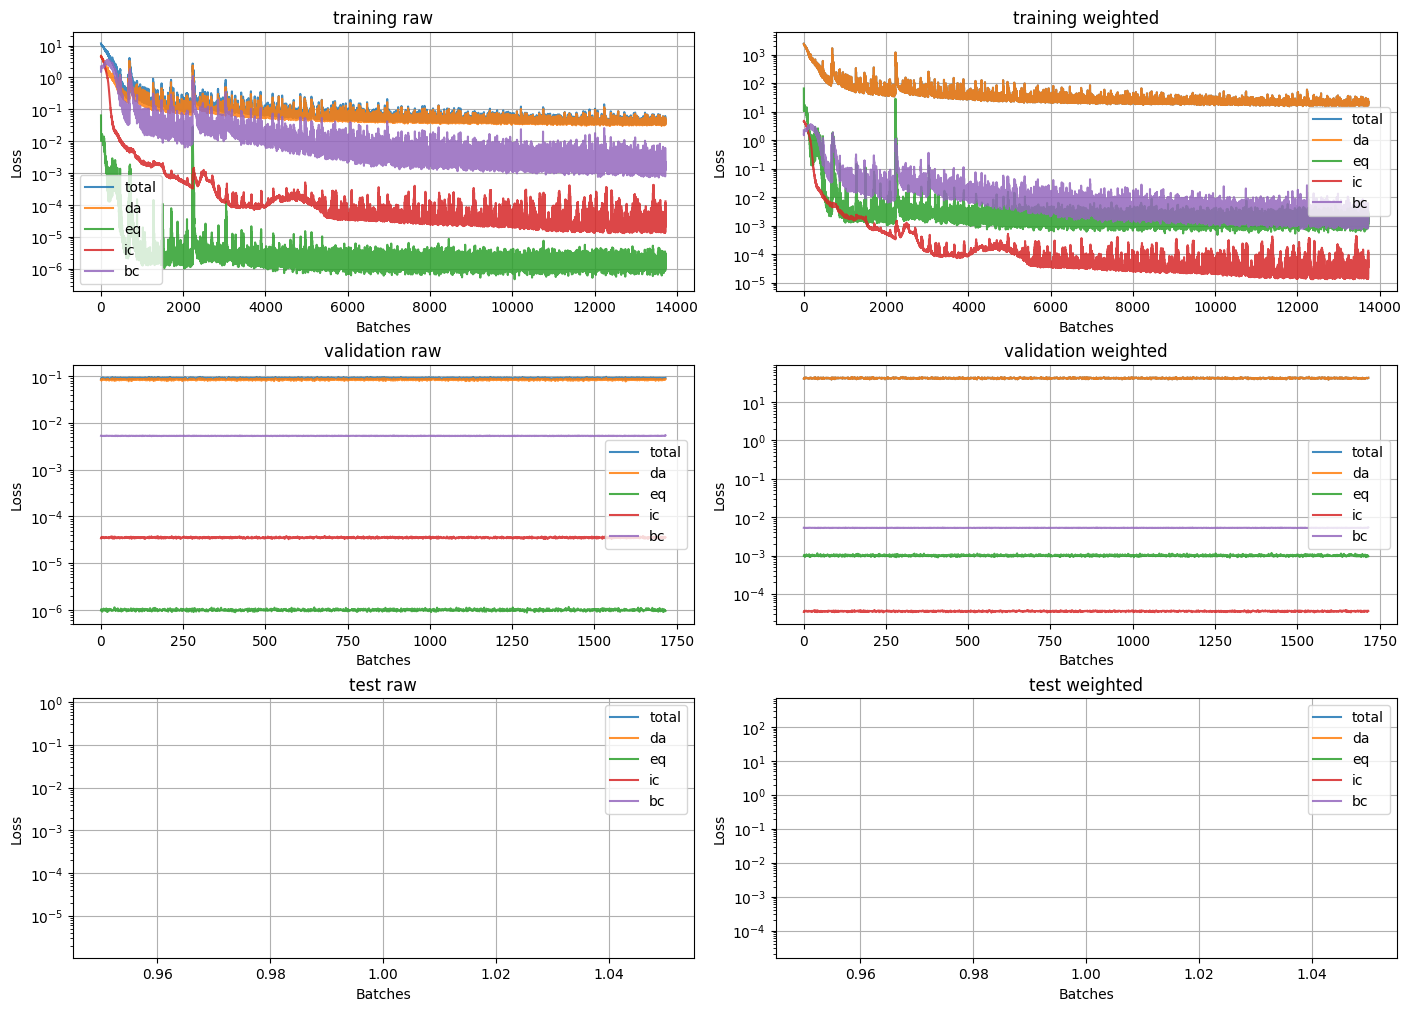
\includegraphics[width=0.8\textwidth]{figures/PINN_træning.png}
     \caption{Endelige eksperimenter for PINN, vægtet og uvægtet loss}
    \label{fig:endelige-traening-composite-loss-for-pinn}
\end{figure}

Her var \texttt{test\_run} den endelige model, der blve trænet og testet.
Den havde en  gennemsnitlig uvægtet test loss på de ukendte datasæt var som følgene:

\begin{table}[H]
    \centering
    \small
    \begin{tabular}{|c|c|c|c|c|c|}
        \hline
        Datasæt & Total loss & Data loss & PDE (eq) loss & IC loss & BC loss \\
        \hline
        \texttt{Alexander\_pi} & $1.531 \cdot 10^{-1}$ & $1.105 \cdot 10^{-1}$ & $5.436 \cdot 10^{-6}$ & $2.575 \cdot 10^{-2}$ & $1.680 \cdot 10^{-2}$ \\
        \texttt{Alexander\_\_fys\_R\_q} & $6.785 \cdot 10^{-1}$ & $2.454 \cdot 10^{-1}$ & $1.687 \cdot 10^{-6}$ & $4.306 \cdot 10^{-1}$ & $2.549 \cdot 10^{-3}$ \\
        \texttt{Alexander\_\_t\_n} & $5.796 \cdot 10^{-1}$ & $5.441 \cdot 10^{-1}$ & $1.237 \cdot 10^{-5}$ & $1.373 \cdot 10^{-3}$ & $3.410 \cdot 10^{-2}$ \\
        \texttt{Alexander\_\_grid\_c\_0} & $6.462 \cdot 10^{-1}$ & $4.723 \cdot 10^{-2}$ & $2.556 \cdot 10^{-6}$ & $5.955 \cdot 10^{-1}$ & $3.420 \cdot 10^{-3}$ \\
        \hline
    \end{tabular}
    \caption{Uvægtede test losses for den endelige PINN model på de ukendte datasæt, opdelt i total loss, data loss, PDE (eq) loss, IC loss og BC loss.}
    \label{tab:pinn-uvægtet-test-loss}
\end{table}


For den endelige visualisering af model prediktion bruges grid da denen har bedste loss.

\begin{figure}[H]
    \centering
    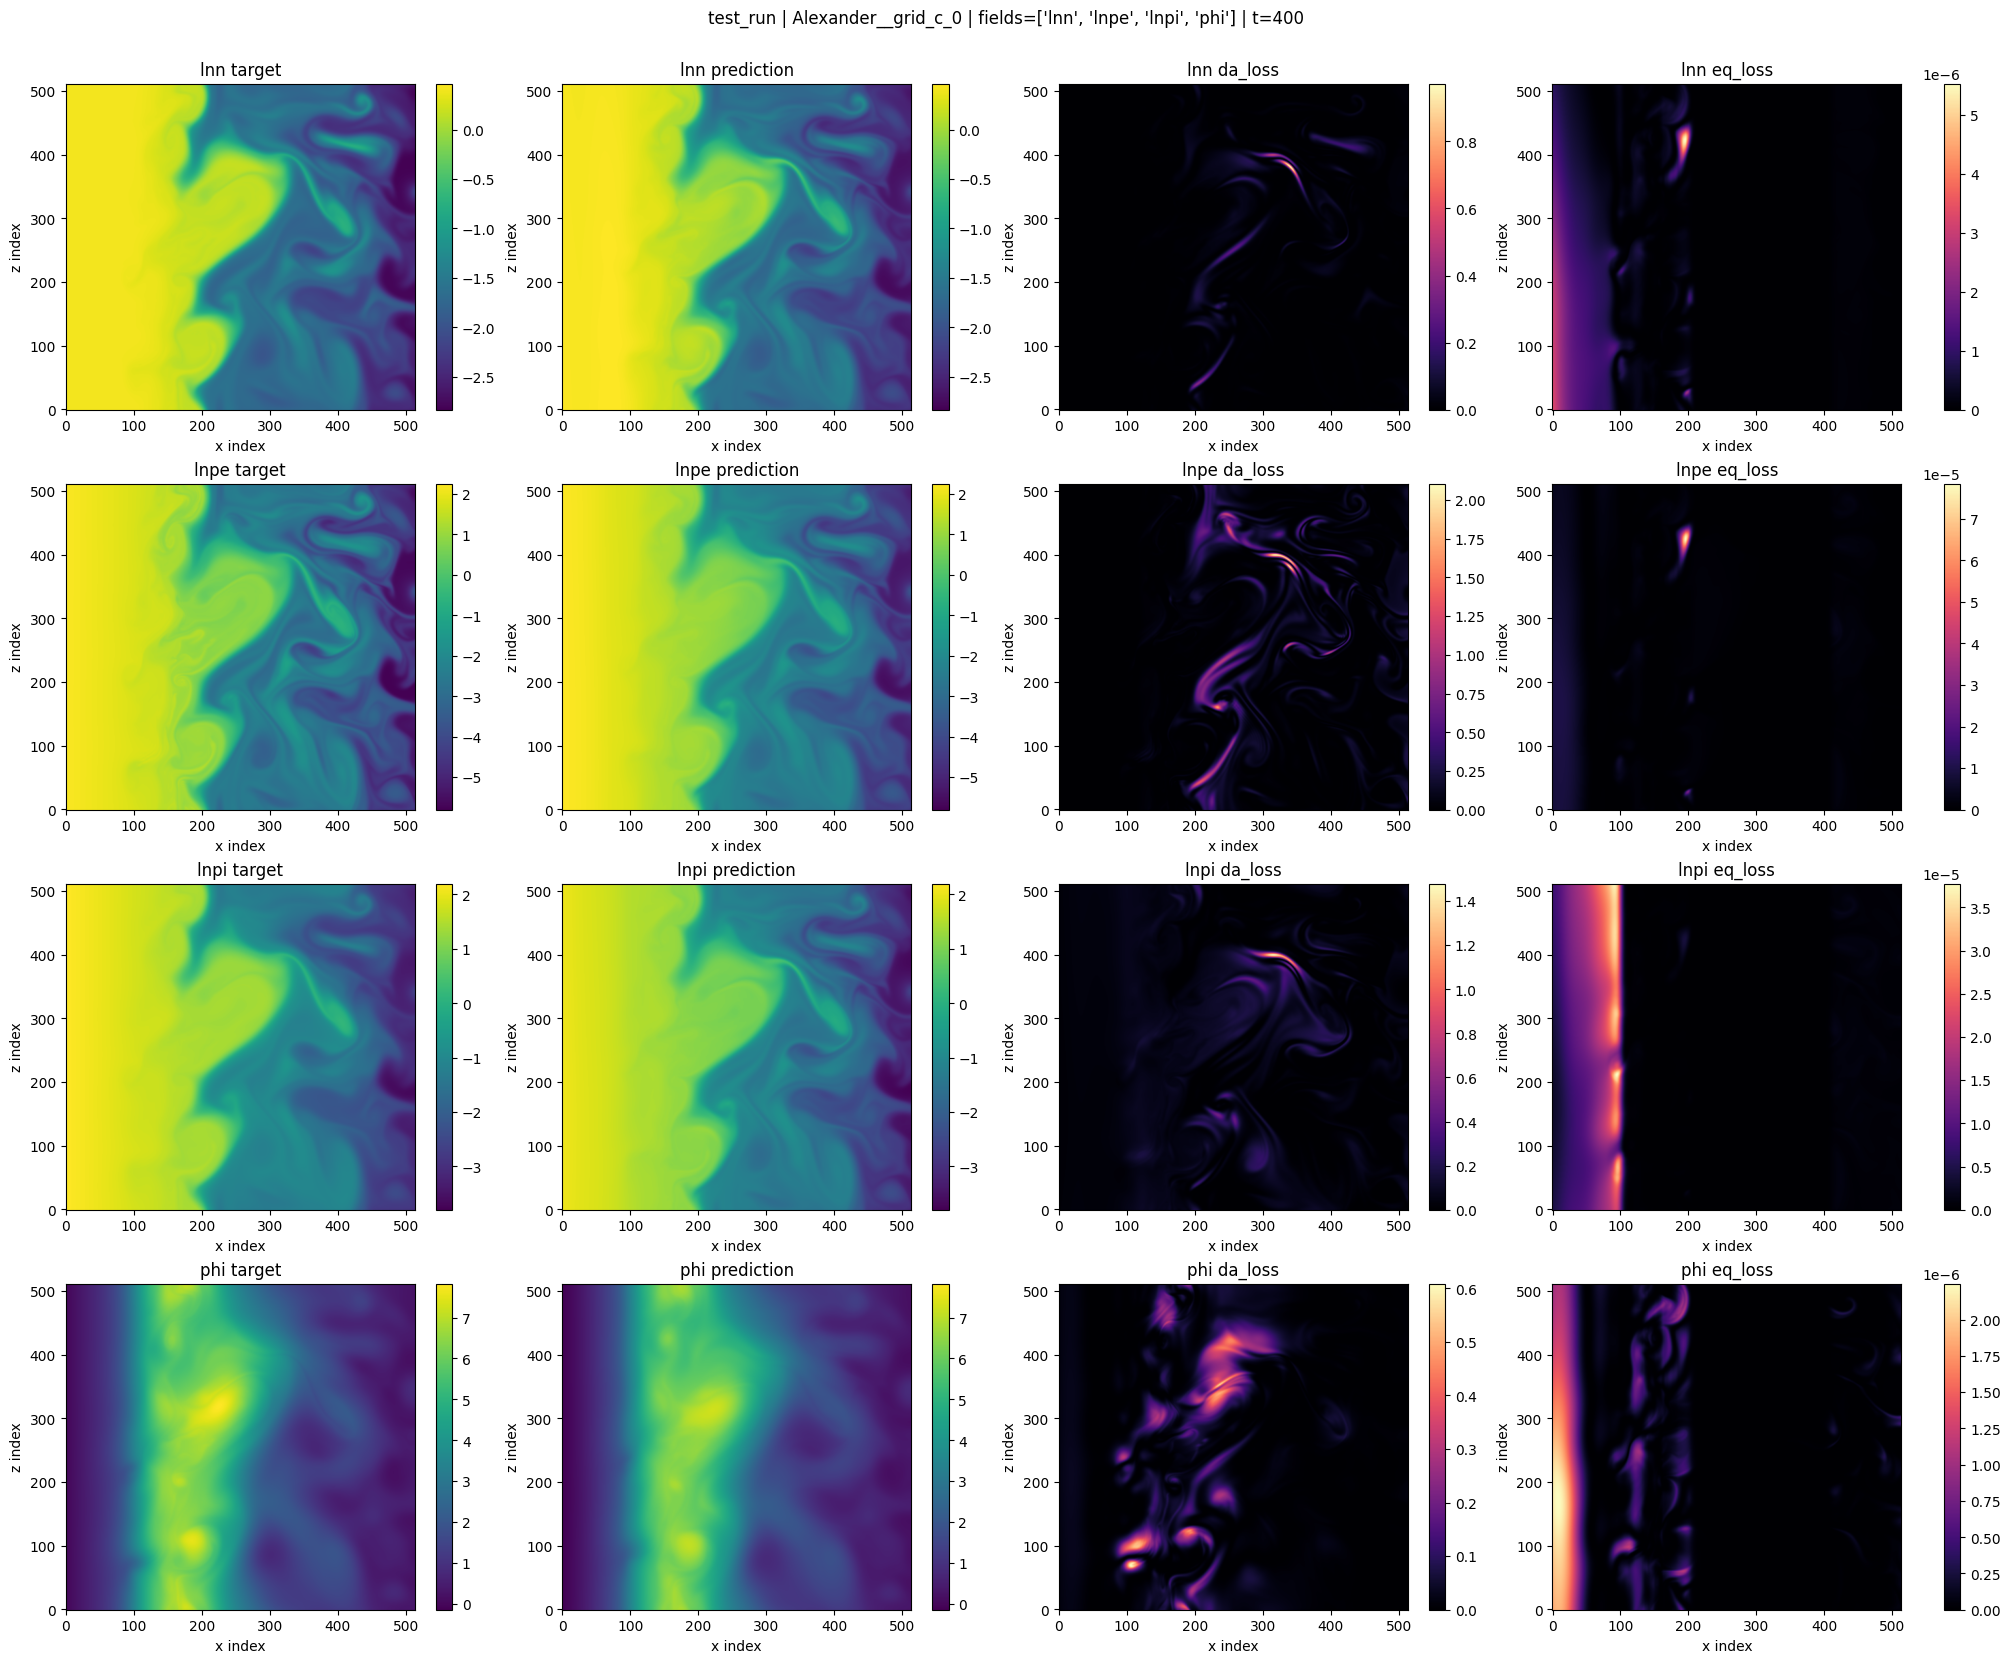
\includegraphics[width=0.8\textwidth]{figures/PINN_final.png}
     \caption{Modellens mål at forudsige \texttt{Alexander\_\_grid\_c\_0} ved \texttt{t\_idx = 400} og \texttt{t\_fys = 00}, sammenlignet med det faktiske resultat, data loss, PDE (eq) loss}
    \label{fig:endelige-prediktion-pinn}
\end{figure}


Det ses på figur \ref{fig:endelige-prediktion-pinn} at modellen rammer meget bedre data dynamikkerne end hvad PINN \_z modellen gjorde.
